\clearpage

\section{bjørnar kladd}

\subsection{web.dev}
lighthouse

PWA: her har bildet en bug, så man får ikke sett scoren, men om man laster ned JSON fil av resultatet, kan man se at den fikk 58\%.
Se json fil. Linje 3386

\subsection{Checkbot}
https://checkbot.io
Funket ikke... klarte ikke å kjøre.
Sendte melding til dev, venter på svar.

\subsection{Color Contrast Analyzer}
\url{https://chrome.google.com/webstore/detail/color-contrast-analyzer/dagdlcijhfbmgkjokkjicnnfimlebcll}

\url{https://accessibility.oit.ncsu.edu/} (North Carolina State University (NC State Uni))

\begin{figure}[H]
    \centering
    \makebox[\textwidth]{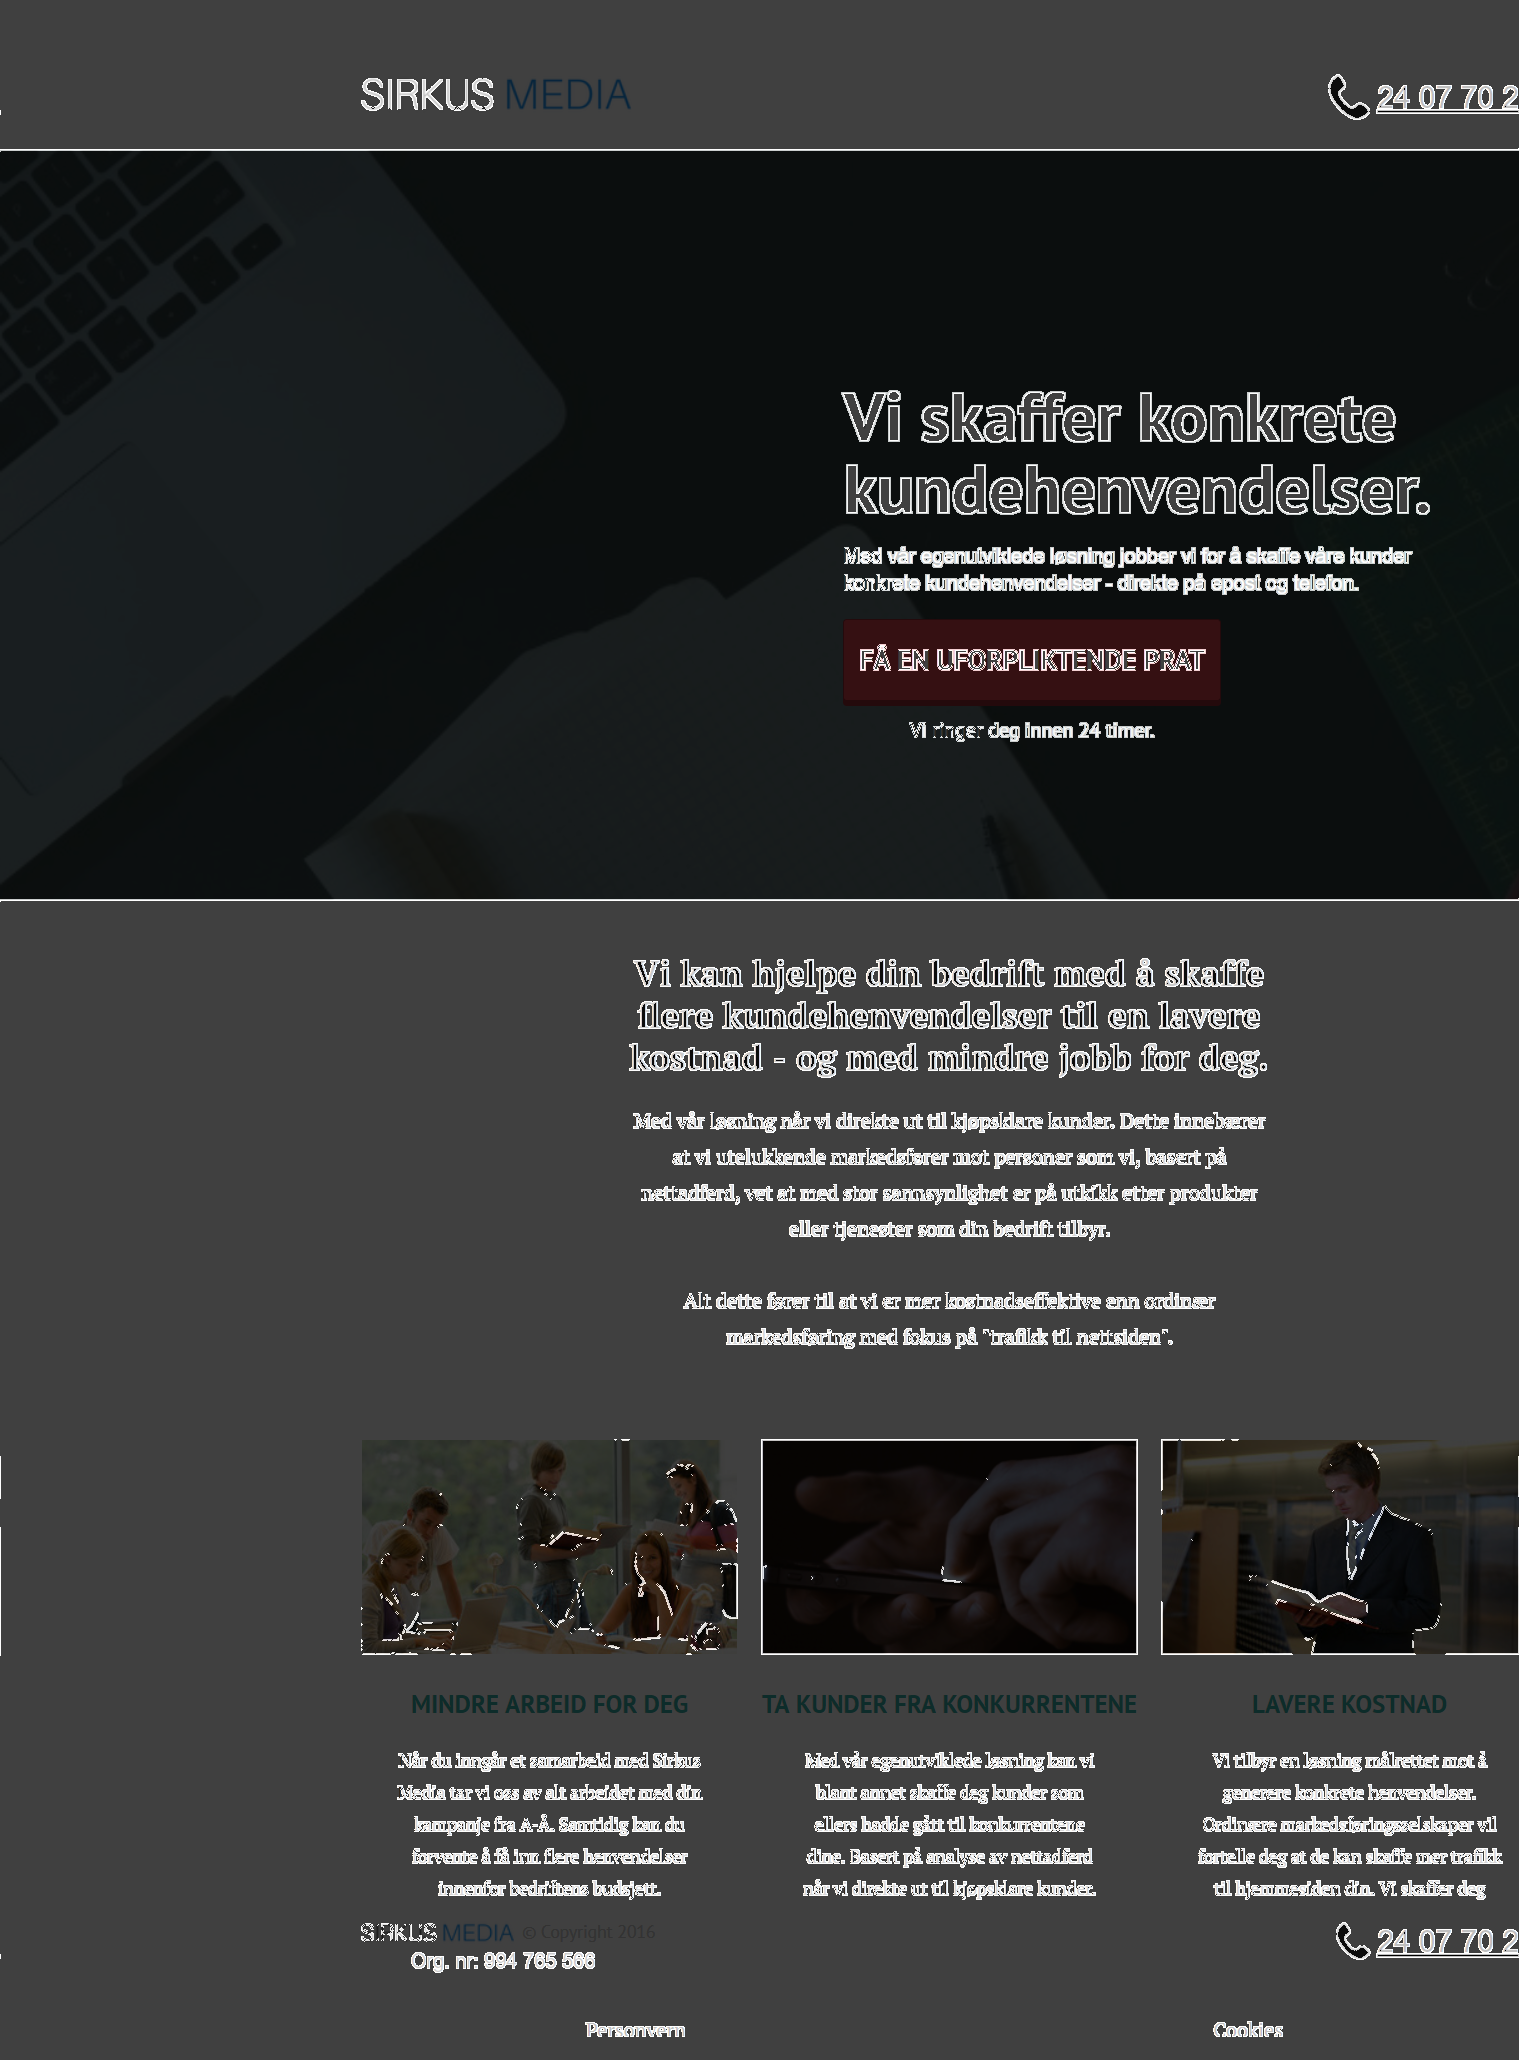
\includegraphics[width=0.80\paperwidth]{bjornar/contrast-wcag-aa-small.png}}
    \caption{CCA resultat AA}
    \label{fig:analysis-current-cca-aa}
\end{figure}

\begin{figure}[H]
    \centering
    \makebox[\textwidth]{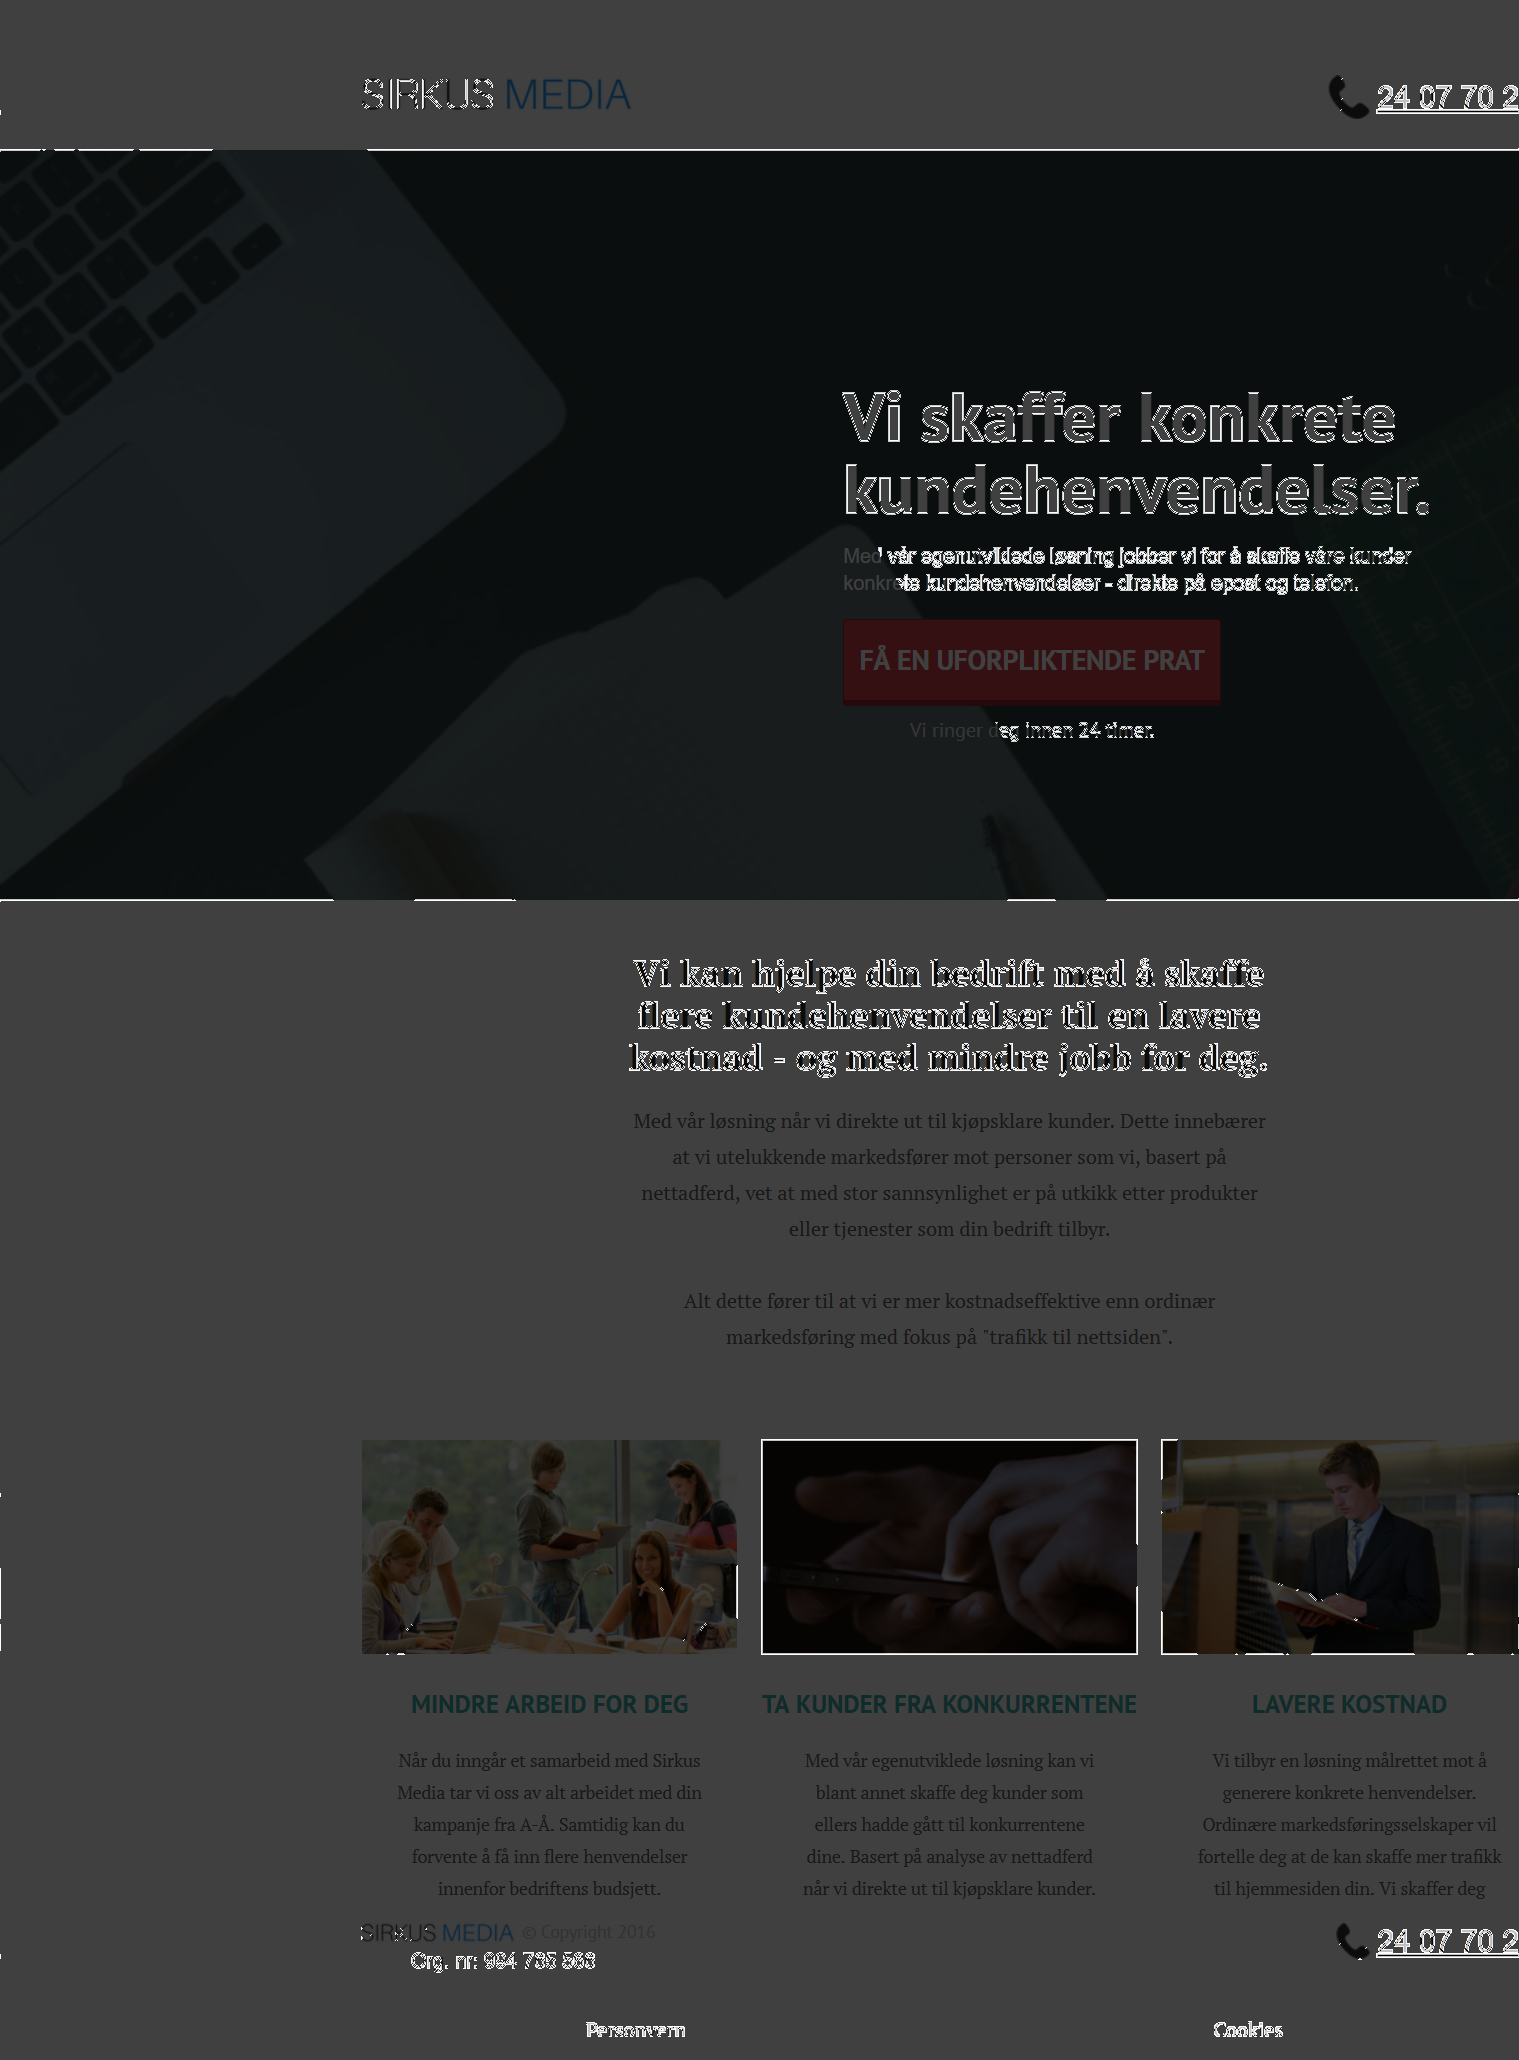
\includegraphics[width=0.80\paperwidth]{bjornar/contrast-wcag-aaa-small.png}}
    \caption{CCA resultat AAA}
    \label{fig:analysis-current-cca-aaa}
\end{figure}

Ser at for Level AA, small non bold text (Se figur \ref{fig:analysis-current-cca-aa}) så failer logo tekst og grønne headings under bildene. Dette kan chrome devtools verifisere. (Se figur \ref{fig:analysis-current-cdt-a} og \ref{fig:analysis-current-cdt-b})

\begin{figure}[H]
    \begin{center}
        \subfigure[grønn overskrift]{\label{fig:analysis-current-cdt-a}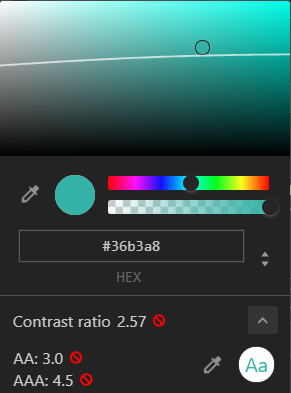
\includegraphics[width=0.3\textwidth]{bjornar/contrast-wcag-aa-small-gronn-tekst.png}}
        \subfigure[blå logo tekst]{\label{fig:analysis-current-cdt-b}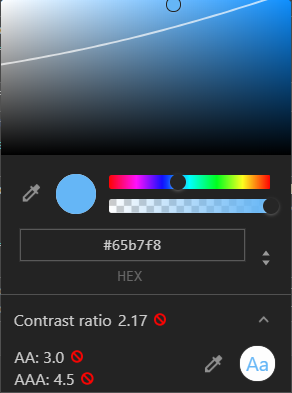
\includegraphics[width=0.3\textwidth]{bjornar/contrast-wcag-aa-small-logo-blaa.png}}
        \subfigure[body tekst]{\label{fig:analysis-current-cdt-c}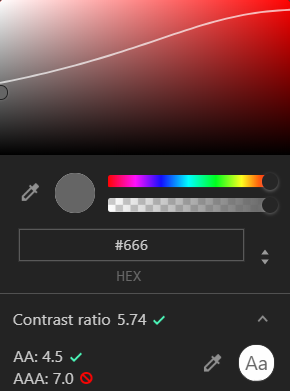
\includegraphics[width=0.3\textwidth]{bjornar/contrast-wcag-aaa-small-body.png}}
        \caption{Chrome devtools - color a11y}
    \end{center}
    
    \label{fig:analysis-current-cdt}
\end{figure}

Når vi tester for Level AAA ser vi at nesten hele siden ikke har bra nok kontrast.
(Se figur \ref{fig:analysis-current-cca-aaa})
Her markeres ikke noe av body teksten på siden.
Tester med chrome devtools, og den kan verifisere resultatet. Se figur \ref{fig:analysis-current-cdt-c}


\subsection{WAVE}
\url{http://wave.webaim.org/}

Kan videre verifisere funnene som ble gjort med verktøy ove (CCA)r. LAG REF.


Når vi skrur på No-styling so ser vi at det er en skjult seksjon på siden.
"THE COMPANIES THAT MAKE THEIR LIFE SIMPLE". Kan plukkes opp av skjermlesere, ikke ideelt.

Andre feil:
1x: Document language missing
4x: Tomme linker
5x: Redudante linker

Annet:
8x: Bilder med tom alt attr.

Bra headings stuktur 
h1: Vi skaffer konkrete kundehenvendelser.
> h2: Vi kan hjelpe din bedrift med å skaffe flere kundehenvendelser til en lavere kostnad - og med mindre jobb for deg.
> > h3: MINDRE ARBEID FOR DEG
> > h3: TA KUNDER FRA KONKURRENTENE
> > h3: LAVERE KOSTNAD


\subsection{https://www.brandwood.com/a11y/}

Når vi ser på header bilde og tekst i CCA, så ser det ut som om det er bra nok for AA, men ikke helt for AAA.
Dette er vanskelig å verifisere med Chrome dev tools eller WAVE. Disse gir en del false-positive ettersom de ikke har noe bakgrunnsfarge å se på, men et bakgrunnsbilde. Dette klarer de altså ikke å teste.

Da kan vi bruke dette verktøyet.

Verktøyet deler opp bilde, der hvor man har tekst over, i seksjoner og finner gjennomsnittsfargen i hver seksjon. Så sjekkes det kontastforholdet mellom hver sekjson og teksten.
Se figur.


\subsection{Chrome dev tools}
Kan sjekke kontrastforhold.

Nettverk tab kan sjekke hastighet.
DOM: 400ms
Load: 1.25s

\begin{table}[]
\begin{tabular}{lllll}
  & DOM & Load &  &  \\
1 & 398 & 1250 &  &  \\
2 & 501 & 1640 &  &  \\
3 & 422 & 1420 &  &  \\
4 & 387 &  928 &  &  \\
5 & 375 & 1720 &  & 
\end{tabular}
\end{table}


\subsection{GOOGLE TRANSPARENCY REPORT - Safe Browsing: malware and phishing}
\url{https://transparencyreport.google.com/safe-browsing/search?url=https://sirkusmedia.no&hl=en-US}

Ingenting funnet

\subsection{SSL test}

\url{https://www.ssllabs.com/ssltest/}


\clearpage